\chapter{Experimental evaluation}
\label{ch:experiments}

In this chapter, we want to evaluate our dynamic algorithms for Top-k closeness centrality and group closeness. 

\section{Graphs}
We evaluate our dynamic algorithms on complex networks from the \emph{Stanford Large Network Dataset Collection}~\cite{snapnets} and on street networks from several countries. We have generated the undirected street networks from the directed source file by assuming directed edges to be undirected and then filtering out duplicate edges.

\begin{table}[h!]
\parbox{.45\linewidth}{
\centering
\begin{tabular}{lrr}

\hline
 Graph                &   Nodes &    Edges \\
\hline
 facebook\_combined    &    4039 &    88234 \\
 ca-GrQc              &    5242 &    14496 \\
 as20000102           &    6474 &    13895 \\
 ca-HepTh             &    9877 &    25998 \\
 oregon1\_010526       &   11174 &    23409 \\
 oregon2\_010526       &   11461 &    32730 \\
 ca-HepPh             &   12008 &   118521 \\
 ca-AstroPh           &   18772 &   198110 \\
 ca-CondMat           &   23133 &    93497 \\
 as-caida20071105     &   26475 &    53381 \\
 email-Enron          &   36692 &   183831 \\
 loc-brightkite\_edges &   58228 &   214078 \\
 loc-gowalla\_edges    &  196591 &   950327 \\
 com-dblp      &  317080 &  1049866 \\
 com-amazon    &  334863 &   925872 \\
 com-youtube   & 1134890 &  2987624 \\
 as-skitter           & 1696415 & 11095298 \\
\hline
\end{tabular}
\caption{Undirected complex networks}

}
\hfill
\parbox{.45\linewidth}{
\centering
\begin{tabular}{lrr}
\hline
 Graph            &   Nodes &   Edges \\
\hline
 wiki-Vote        &    7115 &   103689 \\
 cit-HepTh        &   27770 &   352807 \\
 cit-HepPh        &   34546 &   421578 \\
 p2p-Gnutella31   &   62586 &   147892 \\
 soc-Epinions1    &   75879 &   508837 \\
 twitter\_combined &   81306 &  1768149 \\
 soc-Slashdot0902 &   82168 &   948464 \\
 email-EuAll      &  265214 &   420045 \\
 web-Stanford     &  281903 &  2312497 \\
 web-NotreDame    &  325729 &  1497134 \\
 web-BerkStan     &  685230 &  7600595 \\
 web-Google       &  875713 &  5105039 \\
 wiki-Talk        & 2394385 &  5021410 \\
 cit-Patents      & 3774768 & 16518948 \\
\hline
\end{tabular}

\caption{Directed complex networks and web graphs}
}
\end{table}

\begin{table}[h!]
\centering
\begin{tabular}{lrrr}
\hline
 Graph         &   Nodes &   Edges &   Diameter \\
\hline
 faroe-islands &   31097 &   31974 &       1464 \\
 liechtenstein &   54972 &   56616 &       2176 \\
 isle-of-man   &   61082 &   63793 &       1089 \\
 malta         &   91188 &  101437 &        591 \\
 belize        &   96977 &  103198 &       3242 \\
 azores        &  237174 &  243185 &       1804 \\
\hline
\end{tabular}
\caption{Street networks}
\label{tbl:streetNetworks}

\end{table}


\FloatBarrier

\section{Dynamic Top-k closeness centrality}
First, we want to evaluate our dynamic algorithm for Top-k closeness centrality. We compare our algorithm to the na\"ive approach of simply running the static algorithm again after the graph has changed. We have made our algorithms available through the Python interface of NetworKit and have used Python scripts to collect the data for our experiments. For these experiments, we have used two identical machines with 48 AMD Opteron 6172 cores (clocked at 2.10 GHz) and 256 GB of main memory.

\subsection{Methodology}
Our experiments cover several ``dimensions'':

\begin{itemize}
	\item Edge insertions and edge removals
	\item Directed and undirected graphs
	\item Complex networks and street networks
	\item Different values for $k$
\end{itemize}

\paragraph{Edge insertions}
For our edge insertion experiments, we select 100 edges at random from the base graph and remove them. The resulting graph is the initial graph on which we initialize the dynamic algorithm. We then add back the removed edges one-by-one and measure the update time of the dynamic algorithm. We also create a separate instance of the algorithm and measure the time it requires to run the static algorithm after each edge insertion as a reference. With the update time and the reference time, we can compute the speedup of the dynamic algorithm compared to the static algorithm. In the process, we also collect information about the effectiveness of the various optimization strategies for complex networks we have proposed in Section~\ref{sec:dynamicTopKOptimizations}. In all our experiments, we compare our dynamic algorithm with the static one with $k = 1, 10, 100$.

\paragraph{Edge removals}
To measure the speedup of our dynamic algorithm for edge removals, we start with the base graph. We select 100 edges at random and remove them one-by-one. After each edge removal, we perform the update of the dynamic algorithm and measure the time it takes. We also measure the reference time of the static algorithm and compute the speedup of the dynamic algorithm.

\subsection{Edge insertions in complex networks}
The results for edge insertions in undirected complex networks are shown in Table~\ref{tbl:topkUndirectedComplex}, the results for directed complex networks in Table~\ref{tbl:topkDirectedComplex}. We always yield a double-digit speedup in the geometric mean in undirected networks with $k = 1, 10, 100$.

We achieve smaller speedups on directed networks. One reason for this is the computation of the number of reachable nodes. In the undirected case, computing the number of reachable nodes does not take a significant amount of time in the first place. On top of that, we have a simple optimization for edge insertions which is faster than recomputing the connected components of a graph from scratch. However, in the directed case, computing the upper bound for the number of reachable nodes takes a significant amount of time. For instance, it takes about 2 seconds to do so on the graph \texttt{wiki-Talk}. Since we have not implemented any optimizations for dynamic graphs, this effectively results in a lower bound for the update time in these graphs, even if almost no node is actually affected by an edge insertion.

\paragraph{Update time distribution}
Figures~\ref{fig:updateTimesAs20000102} and \ref{fig:updateTimesAmazon} contain the update times for all 100 inserted edges in the graphs \texttt{as20000102} and \texttt{com-amazon}. In general, the graphs for the undirected complex network we have tested look quite similar. In each case, every update of the dynamic algorithm is faster than running the static algorithm again. For many nodes, the dynamic update is significantly faster. However, there are pathological cases where the update time is close to the static reference time for many graphs. 

\begin{figure}[h!]
  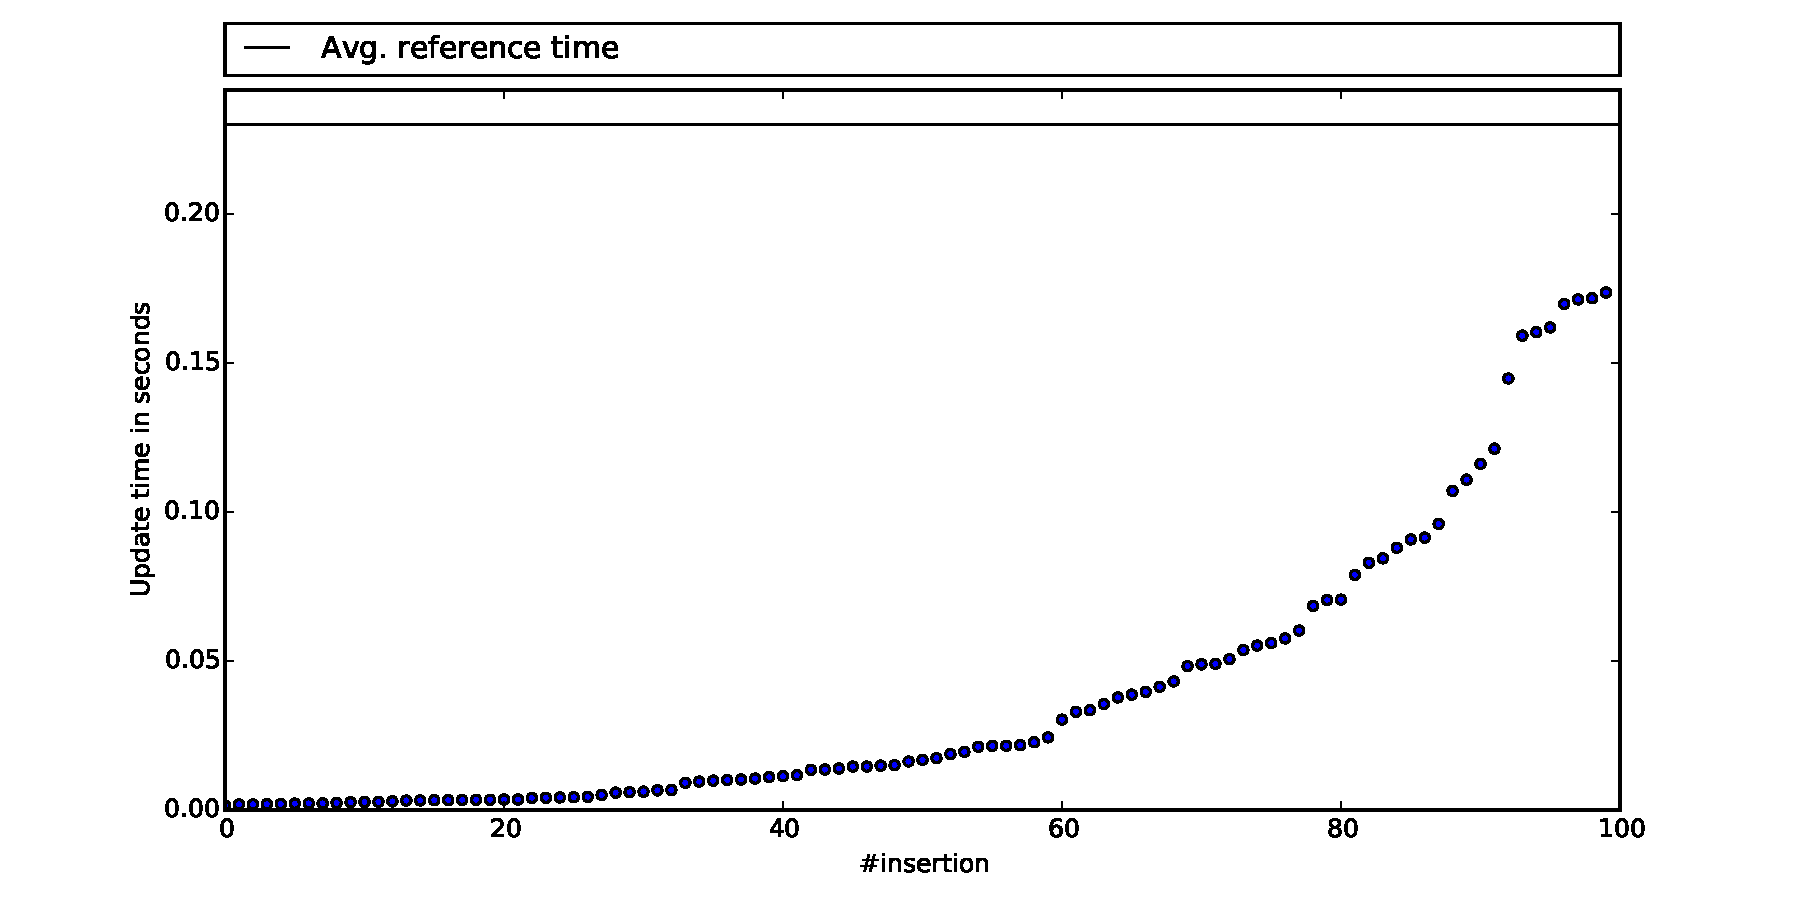
\includegraphics[width=0.95\textwidth]{figures/as20000102_10}
  \caption{Update times of 100 random edge insertions on \texttt{as20000102} with $k = 10$}
  \label{fig:updateTimesAs20000102}
\end{figure}


\begin{figure}[h!]
  \includegraphics[width=0.95\textwidth]{figures/{com-amazon.ungraph_100}.pdf}
  \caption{Update times of 100 random edge insertions on \texttt{com-amazon} with $k = 100$}
  \label{fig:updateTimesAmazon}
\end{figure}

\paragraph{Optimizations}
We now want to examine the effect of the various optimizations we have proposed for the dynamic algorithm for complex networks. Table~\ref{tbl:optimizationImpact} contains the average number of affected nodes and the percentage of nodes skipped due to each of the optimizations. In any case, skipping far-away nodes allows us to ignore the vast majority of affected nodes after an update. Combined with the cheap updates for boundary nodes and applying the level-based improvement bounds, we need to run a new pruned BFS for less than 1\% of the affected nodes in most cases.

\begin{table}[h!]
\begin{tabular}{lrrllll}
\toprule
 Graph                &   affected &   $|V|$ & far-away   & boundary   & impr. bound   & pruned BFS   \\
\midrule \midrule
 as-caida20071105     &       4265 &   26475 & 88.568\%    & 10.934\%    & 0.460\%        & 0.038\%   \\
 as-skitter           &      84560 & 1696415 & 89.475\%    & 9.609\%     & 0.569\%        & 0.347\%   \\
 as20000102           &       1544 &    6474 & 77.106\%    & 16.879\%    & 5.875\%        & 0.141\%   \\
 ca-AstroPh           &        356 &   18772 & 88.659\%    & 6.856\%     & 2.402\%        & 2.084\%   \\
 ca-CondMat           &       3478 &   23133 & 88.338\%    & 4.083\%     & 7.293\%        & 0.287\%   \\
 ca-GrQc              &        625 &    5242 & 86.027\%    & 6.904\%     & 5.917\%        & 1.152\%   \\
 ca-HepPh             &        463 &   12008 & 91.679\%    & 4.472\%     & 2.733\%        & 1.116\%   \\
 ca-HepTh             &       1895 &    9877 & 84.123\%    & 3.530\%     & 11.300\%       & 1.046\%   \\
 com-amazon.ungraph   &      67011 &  334863 & 83.707\%    & 3.611\%     & 12.281\%       & 0.402\%   \\
 com-dblp.ungraph     &      33542 &  317080 & 85.622\%    & 4.115\%     & 10.061\%       & 0.201\%   \\
 com-youtube.ungraph  &     108705 & 1134890 & 67.154\%    & 10.968\%    & 21.362\%       & 0.516\%   \\
 email-Enron          &       1774 &   36692 & 93.648\%    & 5.568\%     & 0.752\%        & 0.032\%   \\
 facebook\_combined    &        274 &    4039 & 73.131\%    & 15.058\%    & 11.545\%       & 0.266\%   \\
 loc-brightkite\_edges &       5557 &   58228 & 65.051\%    & 12.502\%    & 21.411\%       & 1.036\%   \\
 loc-gowalla\_edges    &      10250 &  196591 & 97.420\%    & 2.371\%     & 0.162\%        & 0.047\%   \\
 oregon1\_010526       &       2578 &   11174 & 77.314\%    & 17.255\%    & 5.337\%        & 0.093\%   \\
 oregon2\_010526       &       1409 &   11461 & 83.951\%    & 14.954\%    & 1.004\%        & 0.091\%   \\
\bottomrule
\end{tabular}
\caption{Impact of optimizations}{Analysis of the various optimization strategies, averaged over 100 random edge insertions in undirected complex networks with $k = 10$. The column ``affected'' contains the average number of affected nodes, ``far-away'' the number of nodes skipped because their previous cutoff level was smaller than the distance to the edge insertion, ``boundary'' the number of boundary nodes and ``impr. bound'' the number of nodes that could be updated with their maximum improvement without surpassing the $k$-th most central node.}
\label{tbl:optimizationImpact}
\end{table}

\paragraph{Affected nodes}
We now want to analyze the number of affected nodes after edge modifications. Table~\ref{tbl:optimizationImpact} suggests that, on average, a clear majority of the nodes ($> 80\%$) in the tested graphs are unaffected by a random edge modification. As an example, we have computed the number of affected nodes for each edge in the graph \texttt{oregon1\_010526}. For this purpose, we remove each edge individually from the graph, compute the number of affected nodes and then add the edge back. Figure~\ref{fig:histOregon1} contains a histogram of the data. The median number of affected nodes is 1208 for this graph. The median is represented by the dashed line in the histogram. We can see that for over half of the edges in the graph, only a tenth of all nodes will be affected if the edge is modified. However, there is also a large peak at the other end of the spectrum, where a considerable number of edges affects almost every node in the graph if they are modified. Most of these node have only a single neighbor and removing the edge between them splits the connected component, therefore affecting every node in the connected component.

\begin{figure}[h!]
  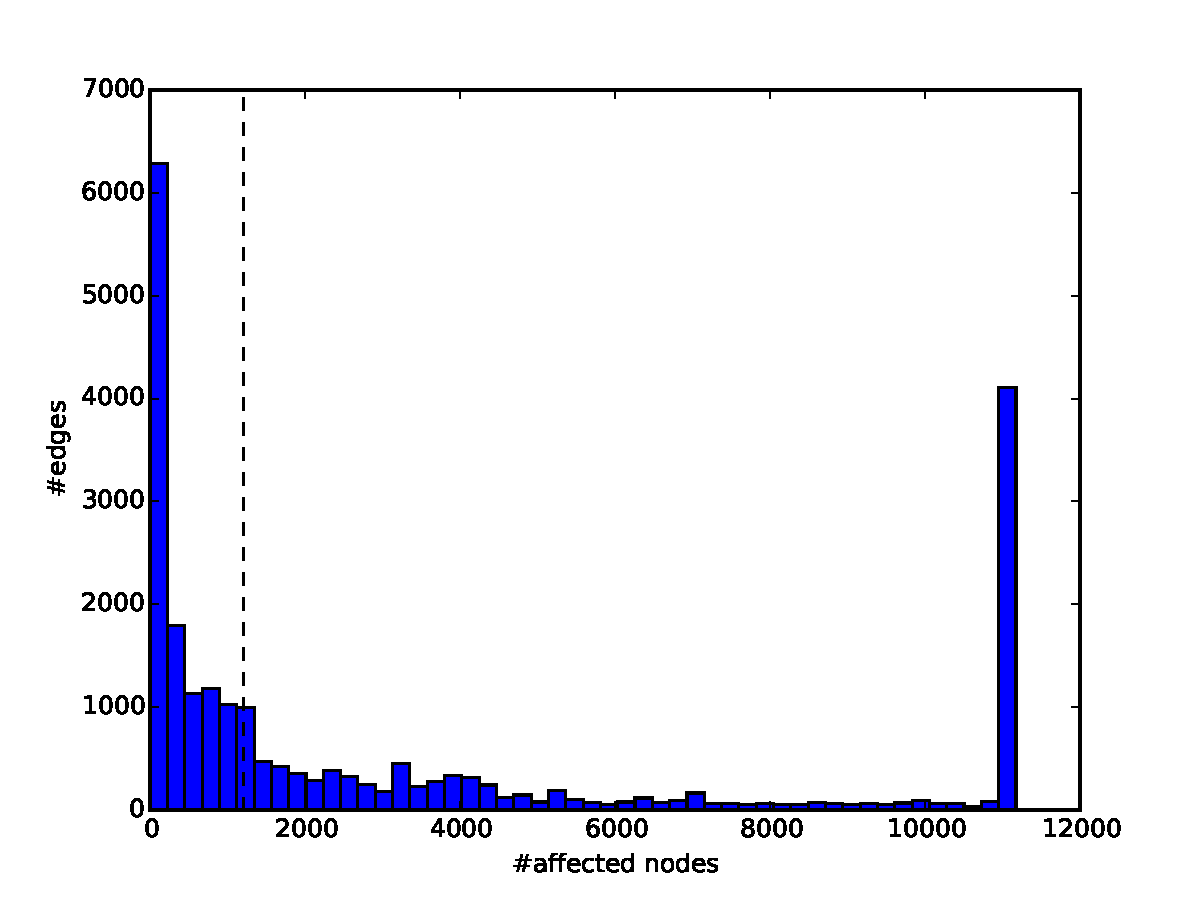
\includegraphics[width=0.95\textwidth]{figures/oregon1-affected}
  \caption{Distribution of the number of affected nodes in \texttt{oregon1\_010526}}
  \label{fig:histOregon1}
\end{figure}

\begin{landscape}

\begin{table}[h]
\centering
\begin{tabular}{l|rrrr|rrrr|rrrr}
\toprule
Graph & \multicolumn{4}{c|}{k = 1} & \multicolumn{4}{c|}{k = 10} & \multicolumn{4}{c}{k = 100}\\
                &     ref [s] &   gmean &   min &     max &     ref [s] &   gmean &   min &     max &     ref [s] &   gmean &   min &     max \\
\midrule \midrule
 facebook\_combined    &   0.132 &  52.354 & 1.729 &  92.226 &   0.13  &  52.961 & 1.671 &  87.422 &   0.13  &  58.617 & 1.519 &  78.683 \\
 ca-GrQc              &   0.182 &  31.932 & 1.909 & 223.006 &   0.187 &  34.259 & 1.919 & 212.018 &   0.18  &  32.648 & 1.905 & 164.15  \\
 as20000102           &   0.225 &  18.163 & 1.34  & 175.157 &   0.23  &  14.219 & 1.182 & 163.056 &   0.22  &  17.367 & 1.349 & 149.471 \\
 ca-HepTh             &   0.335 &  27.743 & 1.56  & 218.97  &   0.341 &  20.706 & 1.483 & 298.27  &   0.33  &  24.422 & 1.482 & 258.957 \\
 oregon1\_010526       &   0.384 &  16.217 & 1.397 & 154.007 &   0.397 &  14.997 & 1.319 & 152.956 &   0.388 &  18.393 & 1.428 & 169.635 \\
 oregon2\_010526       &   0.408 &  31.605 & 1.391 & 178.563 &   0.412 &  39.461 & 1.361 & 174.984 &   0.397 &  33.568 & 1.312 & 148.284 \\
 ca-HepPh             &   0.445 &  60.461 & 2.767 & 331.736 &   0.46  &  60.483 & 1.932 & 123.843 &   0.449 &  58.843 & 1.782 & 114.023 \\
 ca-AstroPh           &   0.675 &  43.052 & 1.376 & 104.393 &   0.703 &  46.843 & 4.032 &  97.165 &   0.762 &  44.18  & 1.992 & 382.766 \\
 ca-CondMat           &   0.804 &  30.455 & 1.473 & 263.041 &   0.821 &  28.09  & 1.455 & 304.707 &   0.81  &  38.934 & 1.495 & 247.589 \\
 as-caida20071105     &   0.955 &  17.172 & 1.283 & 122.889 &   0.967 &  20.043 & 1.451 & 123.456 &   0.933 &  18.087 & 1.236 & 126.564 \\
 email-Enron          &   1.302 &  56.122 & 2.613 & 303.076 &   1.328 &  49.113 & 1.506 & 126.504 &   1.403 &  58.462 & 1.471 & 278.372 \\
 loc-brightkite\_edges &   2.051 &  44.699 & 1.389 & 116.031 &   1.982 &  32.469 & 1.398 & 109.521 &   2.075 &  35.809 & 1.536 & 118.759 \\
 loc-gowalla\_edges    &   7.023 &  52.144 & 1.277 & 111.11  &   8.027 &  53.864 & 1.458 & 112.168 &  22.242 & 107.676 & 1.99  & 322.198 \\
 com-dblp.ungraph     &  11.601 &  17.413 & 1.344 & 112.883 &  12.568 &  31.8   & 1.332 & 117.433 &  17.569 &  33.821 & 1.784 & 151.297 \\
 com-amazon.ungraph   &  27.709 &  38.652 & 2.561 & 214.115 &  33.834 &  45.213 & 2.89  & 220.926 &  99.487 &  88.985 & 9.37  & 726.038 \\
 com-youtube.ungraph  &  29.568 &  20.466 & 1.127 &  84.857 &  88.891 &  68.17  & 2.251 & 190.132 & 124.343 &  68.219 & 3.025 & 290.741 \\
 as-skitter           & 242.991 & 114.884 & 2.35  & 291.879 & 279.276 & 146.953 & 4.849 & 368.249 & 320.279 & 159.128 & 4.519 & 418.5   \\ \midrule \midrule
 (geometric) mean     &  19.223 &  34.231 & 1.631 & 166.282 &  25.327 &  37.686 & 1.798 & 160.411 &  34.823 &  43.355 & 1.932 & 207.488 \\
\bottomrule
\end{tabular}

\caption{Update times for 100 random edge insertions with $k = 1, 10, 100$ in undirected complex networks.  The column ``ref'' contains the average reference time in seconds, ``gmean'' the geometric mean of the achieved speedups, ``min'' and ``max'' the minimum and maximum speedup.}
\label{tbl:topkUndirectedComplex}
\end{table}
\end{landscape}


\begin{landscape}

\begin{table}[h]
\centering
\begin{tabular}{l|rrrr|rrrr|rrrr}
\toprule
Graph & \multicolumn{4}{c|}{k = 1} & \multicolumn{4}{c|}{k = 10} & \multicolumn{4}{c}{k = 100}\\
                &     ref [s] &   gmean &   min &     max &     ref [s] &   gmean &   min &     max &     ref [s] &   gmean &   min &     max \\
\midrule \midrule
 wiki-Vote        &   0.216 &  19.041 & 11.95  & 22.189 &   0.214 &  18.465 & 12.556 &  21.38  &   0.215 &  18     & 8.984 &  21.75  \\
 cit-HepTh        &   0.763 &   8.025 &  1.933 & 10.882 &   0.915 &  11.042 &  1.606 &  14.45  &   0.995 &  11.368 & 4.016 &  14.837 \\
 cit-HepPh        &   0.94  &   9.679 &  1.085 & 13.301 &   0.991 &  10.246 &  1.281 &  14.191 &   1.141 &  11.076 & 1.277 &  15.681 \\
 p2p-Gnutella31   &   1.941 &  12.975 &  3.905 & 23.593 &   1.772 &  11.148 &  3.713 &  18.847 &   2.146 &  11.46  & 3.046 &  21.722 \\
 soc-Epinions1    &   2.273 &  18.292 &  1.279 & 30.288 &   2.311 &  15.941 &  1.442 &  22.304 &   2.419 &  16.37  & 1.215 &  22.423 \\
 soc-Slashdot0902 &   2.566 &  12.678 &  1.038 & 15.689 &   2.762 &  15.008 &  1.208 &  22.42  &   3.84  &  17.313 & 1.585 &  24.955 \\
 twitter\_combined &   2.686 &  11.931 &  1.262 & 15.763 &   2.67  &  12.052 &  1.302 &  14.759 &   4.284 &  17.021 & 1.716 &  20.459 \\
 email-EuAll      &   7.93  &  22.904 &  1.221 & 34.001 &   8.02  &  24.681 &  1.335 &  38.4   &   8.13  &  24.459 & 1.177 &  40.373 \\
 web-NotreDame    &  10.214 &  22.515 &  4.144 & 36.852 &   9.952 &  23.611 &  4.156 &  32.553 &  13.374 &  32.776 & 5.658 &  48.457 \\
 wiki-Talk        &  23.181 &   5.921 &  2.786 & 31.057 &  99.18  &  27.564 & 17.174 &  31.612 & 143.048 &  37.472 & 5.996 &  43.777 \\
 web-Stanford     &  23.433 &  39.419 &  1.319 & 93.015 &  34.845 &  64.707 &  1.277 & 131.088 &  54.918 & 116.648 & 7.278 & 207.119 \\
 web-Google       &  26.529 &  12.369 &  1.13  & 19.26  &  39.589 &  17.832 &  1.584 &  28.016 & 108.569 &  40.943 & 1.588 &  84.751 \\
 cit-Patents      & 151.871 &   9.931 &  8.204 & 11.597 & 153.478 &   9.483 &  7.457 &  11.18  & 159.299 &  10.498 & 8.188 &  13.225 \\ \midrule \midrule
 (geometric) mean &  19.58  &  13.988 &  2.2   & 22.835 &  27.438 &  17.231 &  2.647 &  24.225 &  38.644 &  21.326 & 3.022 &  31.058 \\
\bottomrule
\end{tabular}

\caption{Update times for 100 random edge insertions with $k = 1, 10, 100$ in directed complex networks. The column ``ref'' contains the average reference time in seconds, ``gmean'' the geometric mean of the achieved speedups, ``min'' and ``max'' the minimum and maximum speedup.}
\label{tbl:topkDirectedComplex}
\end{table}
\end{landscape}

\subsection{Edge insertions in street networks}
We now want to evaluate our dynamic algorithm on the six street networks from Table~\ref{tbl:streetNetworks}. We run a similar experiment for street networks as we have for complex networks. The only difference is that we only compute the reference time for ten of the intermediate graphs. We then calculate an average of these reference times and compute the speedups based on the average reference time. The results are listed in Table~\ref{tbl:resultsStreetNetworksUndirected} for the undirected street networks and in Table~\ref{tbl:resultsStreetNetworksDirected} for the directed street networks. We observe that the speedups are generally higher for our street networks than for the complex networks.

One reason for this is that, while many nodes might be affected by an edge insertion, their distance to this graph modification is quite large. Since we have implemented our algorithm for harmonic closeness centrality, the actual closeness centralities of affected nodes do not change by a large amount. This also means that applying the level-based improvement bounds for all affected nodes only rarely results in a new upper bound that is larger than the previous $k$-th largest closeness centrality. In these cases, it is often enough to recompute the exact closeness centralities of the affected nodes among the $k$ most central ones.

We also observe higher average speedups in directed street networks than in undirected street networks. The reason for this is the lower number of affected nodes in directed networks. However, the maximum speedups are generally smaller in the directed networks than in the undirected networks. Since the actual update times are quite small, recomputing the number of reachable nodes becomes a bottleneck and limits the maximum speedup in directed graphs.

\subsection{Edge removals in complex networks}


\begin{landscape}

\begin{table}[h!]
\centering
\begin{tabular}{l|rrrr|rrrr|rrrr}
\toprule
Graph & \multicolumn{4}{c|}{k = 1} & \multicolumn{4}{c|}{k = 10} & \multicolumn{4}{c}{k = 100}\\
                &     ref [s] &   gmean &   min &     max &     ref [s] &   gmean &   min &     max &     ref [s] &   gmean &   min &     max \\
\midrule \midrule
 faroe-islands    &  3.694 &  57.555 & 11.809 & 1018     &  3.462 &  64.882 &  6.235 &  923.889 &  3.475 &  65.796 & 10.89  & 1028.51  \\
 liechtenstein    &  8.965 &  36.632 & 14.685 & 1226.48  &  8.661 &  32.673 & 10.749 &  742.558 &  9.444 &  20.744 &  7.339 & 1443.12  \\
 isle-of-man      & 11.262 &  90.369 & 16.119 & 1499.57  & 11.706 &  74.057 & 22.495 &  282.317 & 11.571 &  53.184 & 14.042 & 1450.95  \\
 malta            & 13.06  & 122.5   & 39.621 & 1080.39  & 12.82  & 118.39  & 27.176 & 1046.01  & 13.603 &  97.763 & 23.099 & 1443.97  \\
 belize           & 20.541 &  62.072 & 21.121 & 1622.32  & 21.712 &  50.048 & 17.789 & 1661.14  & 25.035 &  39.859 & 11.616 & 2019.76  \\
 azores           & 27.199 & 142.13  & 40.248 &  326.176 & 27.247 & 152.377 & 55.461 &  332.258 & 27.915 & 141.379 & 20.682 &  389.911 \\ \midrule \midrule
 (geometric) mean & 14.12  &  76.845 & 21.329 & 1011.4   & 14.268 &  72.208 & 18.526 &  694.093 & 15.174 &  58.478 & 13.564 & 1161     \\
\bottomrule
\end{tabular}
\caption{Update times for 100 random edge insertions with $k = 1, 10, 100$ in undirected street networks. The column ``ref'' contains the average reference time in seconds, ``gmean'' the geometric mean of the achieved speedups, ``min'' and ``max'' the minimum and maximum speedup.}
\label{tbl:resultsStreetNetworksUndirected}
\end{table}

\begin{table}[h!]
\centering
\begin{tabular}{l|rrrr|rrrr|rrrr}
\toprule
Graph & \multicolumn{4}{c|}{k = 1} & \multicolumn{4}{c|}{k = 10} & \multicolumn{4}{c}{k = 100}\\
                &     ref [s] &   gmean &   min &     max &     ref [s] &   gmean &   min &     max &     ref [s] &   gmean &   min &     max \\
\midrule \midrule
 faroe-islands    &  2.604 & 157.908 &  30.16  &  832.939 &  2.728 & 124.944 & 27.203 &  967.669 &  2.866 &  95.685 & 20.759 &  880.479 \\
 liechtenstein    &  8.063 &  71.494 &  30.384 & 1303.71  &  7.826 &  82.943 & 30.561 & 1426.39  &  8.538 &  85.119 & 26.906 & 1588.3   \\
 isle-of-man      &  9.379 & 130.253 &  42.72  & 1531.27  &  9.665 & 145.912 & 22.306 & 1866.73  &  9.668 & 104.827 & 38.813 & 1512.3   \\
 malta            & 11.947 & 191.444 &  27.376 & 1281.98  & 12.332 & 144.149 & 12.984 & 1382.22  & 12.538 & 156.519 & 19.632 & 1091.53  \\
 belize           & 13.906 & 122.54  &  40.854 & 1336.08  & 15.154 &  96.587 &  5.801 & 1007.36  & 16.357 & 120.394 & 29.523 & 1581.21  \\
 azores           & 28.644 & 239.576 & 110.293 &  708.208 & 27.807 & 228.899 & 99.023 &  493.405 & 28.861 & 227.81  & 92.464 &  493.907 \\ \midrule \midrule
 (geometric) mean & 12.424 & 142.191 &  41.113 & 1124.05  & 12.585 & 129.965 & 22.741 & 1099.86  & 13.138 & 124.17  & 32.423 & 1103.21  \\
\bottomrule
\end{tabular}
\caption{Update times for 100 random edge insertions with $k = 1, 10, 100$ in directed street networks. The column ``ref'' contains the average reference time in seconds, ``gmean'' the geometric mean of the achieved speedups, ``min'' and ``max'' the minimum and maximum speedup.}
\label{tbl:resultsStreetNetworksDirected}
\end{table}

\end{landscape}




\begin{landscape}
\begin{table}[h!]
\centering
\begin{tabular}{l|rrrr|rrrr|rrrr}
\toprule
Graph & \multicolumn{4}{c|}{k = 1} & \multicolumn{4}{c|}{k = 10} & \multicolumn{4}{c}{k = 100}\\
                &     ref [s] &   gmean &   min &     max &     ref [s] &   gmean &   min &     max &     ref [s] &   gmean &   min &     max \\
\midrule \midrule
 facebook\_combined    &   0.112 &  11.728 &  3.089 &  15.198 &   0.121 &  12.838 &  4.341 &  16.538 &   0.13  &  13.023 &  3.478 &  17.738 \\
 ca-GrQc              &   0.154 &  47.108 & 10.856 & 921.962 &   0.157 &  41.522 &  8.545 & 915.638 &   0.151 &  33.438 &  8.024 & 760.947 \\
 as20000102           &   0.188 &  33.583 & 15.427 &  43.933 &   0.194 &  26.907 & 13.988 &  46.148 &   0.183 &  19.545 & 11.064 &  43.828 \\
 ca-HepTh             &   0.282 &  35.877 & 11.908 & 852.242 &   0.28  &  30.011 &  7.964 & 847.234 &   0.276 &  23.076 &  7.976 & 784.087 \\
 oregon1\_010526       &   0.321 &  31.173 & 11.265 &  40.368 &   0.32  &  22.73  &  9.516 &  40.944 &   0.318 &  19.128 &  8.211 &  39.713 \\
 oregon2\_010526       &   0.332 &  28.051 & 13.129 &  34.747 &   0.346 &  22.474 &  9.019 &  36.018 &   0.334 &  18.171 & 10.194 &  34.048 \\
 ca-HepPh             &   0.386 &  19.669 &  3.364 & 849.561 &   0.408 &  19.875 &  3.684 & 888.877 &   0.396 &  16.635 &  2.901 & 816.004 \\
 ca-AstroPh           &   0.568 &  17.244 &  4.772 & 767.619 &   0.577 &  17.019 &  3.945 & 709.664 &   0.669 &  16.377 &  2.612 & 829.106 \\
 ca-CondMat           &   0.675 &  24.785 &  9.003 & 737.27  &   0.711 &  23.31  &  7.069 & 733.503 &   0.683 &  18.828 &  6.552 & 698.119 \\
 as-caida20071105     &   0.76  &  22.871 & 10.245 &  31.764 &   0.767 &  18.889 & 11.36  &  32.13  &   0.757 &  14.617 &  9.69  &  31.569 \\
 email-Enron          &   1.053 &  23.66  &  7.163 & 678.557 &   1.075 &  21.952 &  9.441 & 645.415 &   1.173 &  21.828 &  8.032 & 704.578 \\
 loc-brightkite\_edges &   1.674 &  16.77  &  8.169 &  20.462 &   1.689 &  13.874 &  5.888 &  21.335 &   1.803 &  12.232 &  5.648 &  22.23  \\
 loc-gowalla\_edges    &   5.764 &  12.352 &  5.15  &  15.834 &   6.421 &  12.121 &  5.815 &  17.186 &  19.233 &  21.904 &  1.703 &  50.859 \\
 com-dblp      &   9.632 &  12.491 &  3.694 &  18.524 &  10.192 &  10.809 &  3.534 &  19.029 &  15.289 &  11.486 &  3.136 &  28.805 \\
 com-amazon    &  31.525 &  33.324 &  5.763 &  57.895 &  30.694 &  21.648 &  2.658 &  49.403 &  83.667 &  42.646 &  7.778 & 134.251 \\
 com-youtube   &  37.569 &  14.913 &  5.938 &  20.414 &  95.859 &  18.927 &  1.353 &  54.741 & 133.456 &  20.08  &  1.529 &  74.309 \\
 as-skitter           & 336.102 &  53.084 &  1.033 &  84.169 & 313.04  &  35.342 &  1.073 &  76.443 & 492.071 &  39.964 &  1.08  & 121.05  \\
\bottomrule
\end{tabular}
\caption{Update times for 100 random edge removals with $k = 1, 10, 100$ in undirected complex networks. The column ``ref'' contains the average reference time in seconds, ``gmean'' the geometric mean of the achieved speedups, ``min'' and ``max'' the minimum and maximum speedup.}
\end{table}

\end{landscape}


\begin{landscape}

\begin{table}[h!]
\centering
\begin{tabular}{l|rrrr|rrrr|rrrr}
\toprule
Graph & \multicolumn{4}{c|}{k = 1} & \multicolumn{4}{c|}{k = 10} & \multicolumn{4}{c}{k = 100}\\
                &     ref [s] &   gmean &   min &     max &     ref [s] &   gmean &   min &     max &     ref [s] &   gmean &   min &     max \\
\midrule \midrule
 faroe-islands &  3.000     & 174.525 & 46.465 & 2119.15 &  3.03  & 176.409 & 60.66  & 2415.04 &  2.991 & 162.026 & 37.017 & 2076.44 \\
 liechtenstein &  7.842 &  76.118 & 50.133 & 1744.71 &  7.884 &  76.006 & 54.175 & 2248.93 &  8.836 &  73.512 & 54.79  & 2950.11 \\
 isle-of-man   & 10.281 &  84.939 & 67.748 & 3055.96 &  9.977 &  78.024 & 64.428 & 2563.11 & 10.207 &  65.256 & 52.595 & 2689.05 \\
 malta         & 11.597 &  93.482 & 51.771 & 1543.31 & 12.172 &  93.48  & 51.991 & 1430.01 & 12.253 &  83.264 & 47.082 & 1467.43 \\
 belize        & 17.508 & 119.023 & 25.744 & 1950.99 & 17.523 & 112.325 & 20.783 & 2142.72 & 19.817 & 101.253 & 13.732 & 2394.16 \\
 azores        & 25.804 & 220.592 & 38.487 &  890.16 & 25.567 & 230.051 & 39.725 & 1122.2  & 25.241 & 209.382 & 36.414 & 1138.82 \\
\bottomrule
\end{tabular}
\caption{Update times for 100 random edge removals with $k = 1, 10, 100$ in undirected street networks. The column ``ref'' contains the average reference time in seconds, ``gmean'' the geometric mean of the achieved speedups, ``min'' and ``max'' the minimum and maximum speedup.}
\end{table}

\begin{table}[h!]
\centering
\begin{tabular}{l|rrrr|rrrr|rrrr}
\toprule
Graph & \multicolumn{4}{c|}{k = 1} & \multicolumn{4}{c|}{k = 10} & \multicolumn{4}{c}{k = 100}\\
                &     ref [s] &   gmean &   min &     max &     ref [s] &   gmean &   min &     max &     ref [s] &   gmean &   min &     max \\
\midrule \midrule
 faroe-islands &  2.984 & 307.814 & 49.063 & 3755.06  &  3.05  & 312.551 & 54.554 & 3881.59  &  3.119 & 305.6   & 41.437 & 3899.65  \\
 liechtenstein &  8.664 & 166.661 & 60.866 & 3983.57  &  8.64  & 174.874 & 68.587 & 6251.16  &  9.812 & 163.476 & 55.419 & 3834.49  \\
 isle-of-man   & 10.859 & 155.951 & 63.212 &  366.018 & 11.103 & 173.229 & 65.429 &  374.513 & 11.873 & 163.354 & 63.113 &  402.725 \\
 malta         & 12.527 & 202.493 & 49.013 & 4710.48  & 12.535 & 189.714 & 52.262 & 4548.08  & 12.787 & 174.614 & 48.63  & 4333.87  \\
 belize        & 13.146 & 160.658 & 55.867 & 4233.6   & 13.417 & 164.816 & 50.796 & 4483     & 14.241 & 150.264 & 45.17  & 4870.38  \\
 azores        & 32.032 & 565.52  & 43.012 & 2162.45  & 31.112 & 666.809 & 44.899 & 3347.73  & 30.644 & 578.381 & 36.675 & 3259.14  \\
\bottomrule
\end{tabular}
\caption{Update times for 100 random edge removals with $k = 1, 10, 100$ in directed street networks. The column ``ref'' contains the average reference time in seconds, ``gmean'' the geometric mean of the achieved speedups, ``min'' and ``max'' the minimum and maximum speedup.}
\end{table}

\end{landscape}


\section{Group closeness}